\chapter{Case Studies} \label{section:mparser}

\section{General Parser}
This section demonstrates several applications of our general parser combinator library.

\subsection{Arithmetic Expression}
Here is a parser for an arithmetic expression and its generalized version to provide a glimpse of how to use the library.

An arithmetic expression can be constructed by an integer (we do not consider any floating numbers here), a variable, a function call and several operators with predefined priorities. This data structure can be described as follows.

\begin{lstlisting}
data Expr = Con Int
          | Var CharList
          | Fun CharList PolyList[Expr]
          | Add Expr Expr
          | Min Expr Expr
          | Mul Expr Expr
          | Div Expr Expr;
\end{lstlisting}

This grammar can be split into two components. The first one is \texttt{factor} which contains a constant, a variable, a function call or an expression and is separated by '*' or '/'.  The second one is \texttt{term} which contains \texttt{factors} and is separated by '+' or '-'.
To parse this grammar, we will define three combinators by combining the existing combinators in our library. The first combinator is called \texttt{fact} which designed to parse a factor. The second combinator is called \texttt{term} that is to parse a term. The third combinator is \texttt{expr} that parses the expression as a whole. These three parsers are shown as below.

\begin{lstlisting}
let rec fact: Parser[Char, Expr] =
    \(cs: CharList) -> (
        (integer <@[Char, Int, Expr] (\(v: Int) -> Con v))
        <|>[Char, Expr] ((identifier
            ~[Char, CharList, (CharList -> Expr)]
                (option[Char, PolyList[Expr]] (parenthesized[PolyList[Expr]] (commaList[Expr] expr))
                <?@[Char, PolyList[Expr], (CharList -> Expr)]
                (\(cs: CharList) ->
                    Var cs, (
                        flip[CharList, PolyList[Expr], Expr]
                            (\(cs: CharList) ->
                              \(pl: PolyList[Expr]) -> Fun cs pl)))))
        <@[Char, (CharList, (CharList -> Expr)), Expr]
            (\(v: (CharList, (CharList -> Expr))) -> v._2 v._1))
    <|>[Char, Expr] (parenthesized[Expr] expr)) cs
and term: Parser[Char, Expr] =
    \(cs: CharList) ->
        (chainr[Char, Expr] fact (symbol '*'
            <@[Char, Char, (Expr -> Expr -> Expr)]
            (\(c: Char) -> \(a: Expr) -> \(b: Expr) -> Mul a b)
                <|>[Char, (Expr -> Expr -> Expr)]
            (symbol '/' <@[Char, Char, (Expr -> Expr -> Expr)]
                (\(c: Char) -> \(a: Expr) -> \(b: Expr) -> Div a b)))) cs
and expr: Parser[Char, Expr] =
    \(cs: CharList) ->
        (chainr[Char, Expr] term (symbol '+'
            <@[Char, Char, (Expr -> Expr -> Expr)]
            (\(c: Char) -> \(a: Expr) -> \(b: Expr) -> Add a b)
                <|>[Char, (Expr -> Expr -> Expr)]
            (symbol '-' <@[Char, Char, (Expr -> Expr -> Expr)]
                (\(c: Char) -> \(a: Expr) -> \(b: Expr) -> Min a b)))) cs;
\end{lstlisting}

Now we can just use \texttt{expr} to parse the arithmetic expressions read by the function \texttt{readPolyList} defined in the source code file. In order to test it, we write a Python script which reads each line of the test cases provided and inserts them into the last line of copied parser source code. Then, it invokes all the parsers respectively via the command line to parse the test cases. The figure below demonstrates the testing result.
\begin{figure}[htbp]
    \centering
    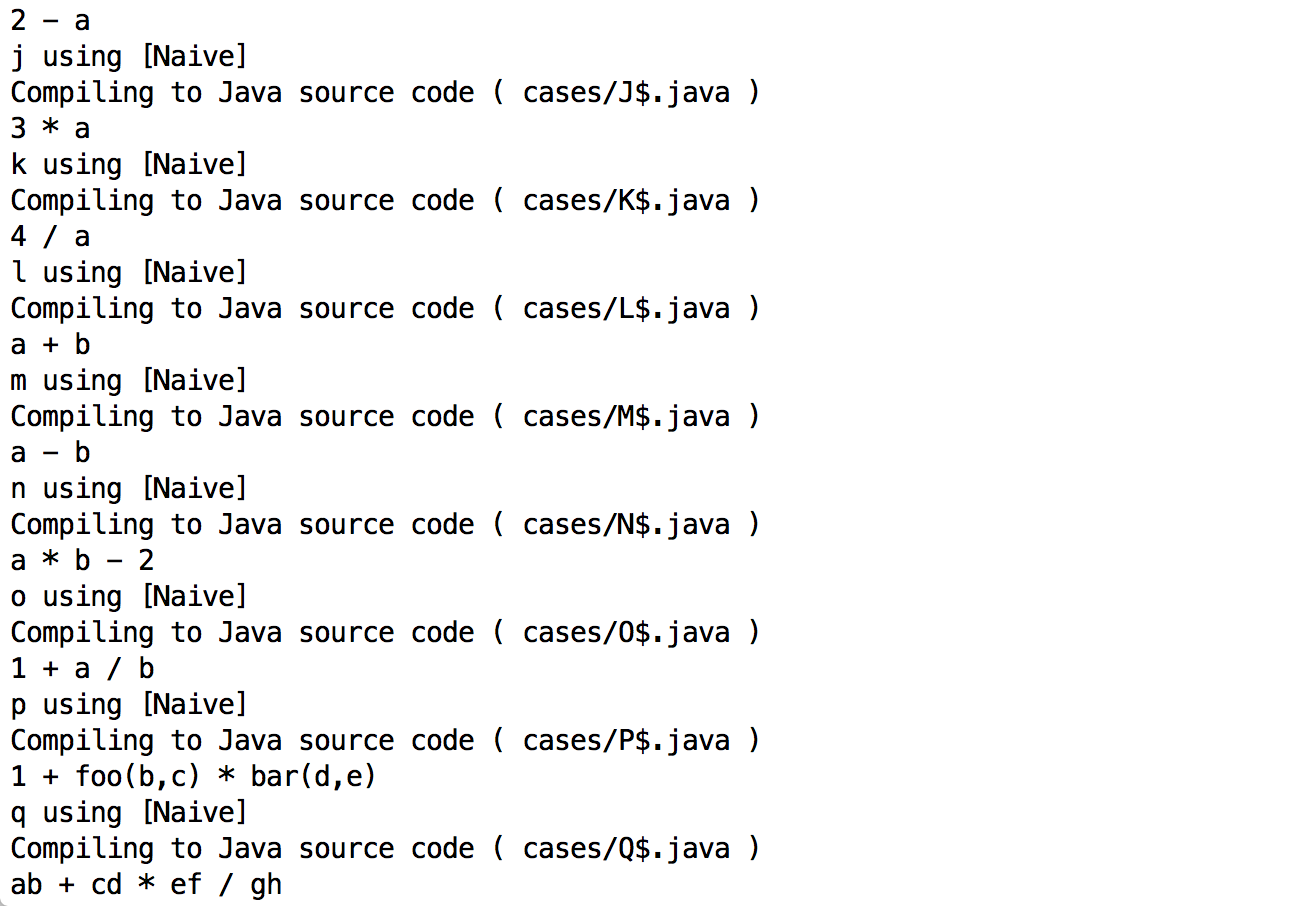
\includegraphics[width=0.7\textwidth]{imgs/general_test}
    \caption{Tests for Arithmetic Expressions}
    \label{fig:general arithmetic}
\end{figure}

However, this combinator only suites for expressions with '+', '-', '*', '/' operations. To generalize it, we can define a parser that can parse any expressions containing any predefined operations with different priorities. This task is relatively easy thanks to the combinators in the library. We firstly define an operation type \texttt{Op} which is a tuple that contains a symbol of operation and its behavior. Then we define a combinator \texttt{gen} that accepts such operations and a parser, and applies the operation on the parsing result. By using \texttt{gen}, we can change our arithmetic expression parser into the below format with some helper combinators introduced.

\begin{lstlisting}
type Op[A] = (Char, A -> A -> A);

let gen[A] (ops: PolyList[Op[A]]) (p: Parser[Char, A]): Parser[Char, A] =
    chainr[Char, A] p (choice[Char, (A -> A -> A)]
        (map[Op[A], Parser[Char, (A -> A -> A)]]
            (\(op: Op[A]) ->
                (symbol op._1 <@[Char, Char, (A -> A -> A)]
                  (\(c: Char) -> op._2))) ops));

let multis: PolyList[Op[Expr]] = Cons[Op[Expr]] ('*',
  \(a: Expr) ->
  \(b: Expr) -> Mul a b) (Cons[Op[Expr]] ('/', \(a: Expr) ->
  \(b: Expr) -> Div a b) (Nil[Op[Expr]]));

let addis: PolyList[Op[Expr]] = Cons[Op[Expr]] ('+',
  \(a: Expr) ->
  \(b: Expr) -> Add a b) (Cons[Op[Expr]] ('-', \(a: Expr) ->
  \(b: Expr) -> Min a b) (Nil[Op[Expr]]));

let expr1: Parser[Char, Expr] = foldr[PolyList[Op[Expr]], Parser[Char, Expr]] (gen[Expr])
  fact (Cons[PolyList[Op[Expr]]]
    addis
        (Cons[PolyList[Op[Expr]]]
            multis
                (Nil[PolyList[Op[Expr]]])));
\end{lstlisting}

The parser \texttt{expr1} does the same thing as \texttt{expr} but this way it is combined with generalized combinators. We can also parse other kinds of expressions by providing self-defined operations. To parse a more complicated grammar with possible variables bindings, we will introduce a skeleton in the next section.

\subsection{Self Application}
As for a given string that follows BNF grammar, we can build a parser to parse all this kinds of strings. Things we need to do are firstly defining a type to associate variables under certain environment and implementing combinators that parse different components of a BNF string.

First things first. We define a type called \texttt{Env} as a series of tuples with the first element denoting a key and the second one its value. To bind a variable and its value, we use a helper function called \texttt{assoc}. And to apply some operations on all variables in an environment, we define a \texttt{mapenv} to realize it. These implementations are listed below.

\begin{lstlisting}
type Env[A, B] = PolyList[(A, B)];
let rec assoc[D] (env: Env[Symbol, D]) (s: Symbol) (default: D): D =
    case env of
        Nil       -> default
    |   Cons e es -> if (e._1 <==> s) then e._2 else (assoc[D] es s default);

let rec mapenv[S, A, B] (f: A -> B) (env: Env[S, A]): Env[S, B] =
    case env of
        Nil       -> Nil[(S, B)]
    |   Cons e es -> Cons[(S, B)] (e._1, f e._2) (mapenv[S, A, B] f es);
\end{lstlisting}

BNF grammar contains either terminal words or non-terminal words. By abstracting it, we use a data type \texttt{Symbol} to represent it. The right hand side of the production rule must be a series of possibilities, each of which is a list of symbols. Hence, the grammar \texttt{Gram} can be represented as below.

\begin{lstlisting}
data Symbol = Term CharList
            | Nont CharList;
type Alt = PolyList[Symbol];
type Rhs = PolyList[Alt];
type Gram = Env[Symbol, Rhs];
\end{lstlisting}

Based on these types, now we can build a parser \texttt{bnf} to parse a BNF string by combining combinators in the library together.

\begin{lstlisting}
let bnfTerm (termp: Parser[Char, CharList]): Parser[Char, Symbol] =
    sp[CharList] termp <@[Char, CharList, Symbol] (\(cs: CharList) ->
    Term cs);

let bnfNont (nontp: Parser[Char, CharList]): Parser[Char, Symbol] =
    sp[CharList] nontp <@[Char, CharList, Symbol] (\(cs: CharList) ->
    Nont cs);

let alt (termp: Parser[Char, CharList]) (nontp: Parser[Char, CharList]): Parser[Char, Alt] =
    many[Char, Symbol] (bnfTerm termp <|>[Char, Symbol] (bnfNont nontp));

let rhs (termp: Parser[Char, CharList]) (nontp: Parser[Char, CharList]): Parser[Char, Rhs] =
    listOf[Char, Alt, Char] (alt termp nontp) (sp[Char] (symbol '|'));

let rule (termp: Parser[Char, CharList]) (nontp: Parser[Char, CharList]): Parser[Char, (Symbol, Rhs)] =
    (bnfNont nontp) ~[Char, Symbol, Rhs]
        (sp[CharList] (token (readPolyList "::=")) ~>[Char, CharList, Rhs]
        (rhs termp nontp) <~[Char, Rhs, Char] (sp[Char] (symbol '.')));

let bnf (nontp: Parser[Char, CharList]) (termp: Parser[Char, CharList]): Parser[Char, Gram] =
    many[Char, (Symbol, Rhs)] (rule termp nontp);
\end{lstlisting}

Now given a BNF string, we are potentially available to build our own parse tree with parser \texttt{bnf}. But it is a good idea to define a new parse tree for generic application. This data type is called \texttt{GramTree}, a multi-branching tree.

\begin{lstlisting}
data GramTree = Node Symbol (PolyList[GramTree]);
\end{lstlisting}

Then we define a combinator \texttt{parsGram} that parses a symbol, an alternative and the right hand side of a rule. This combinator, again, is implemented by several helper functions.

\begin{lstlisting}
let rec parsSym (gram: Gram) (s: Symbol): Parser[Symbol, GramTree] =
    case s of
        Term t -> symbol2 s <@[Symbol, Symbol, PolyList[GramTree]]
          (\(sym: Symbol) -> Nil[GramTree]) <@[Symbol, PolyList[GramTree], GramTree] (\(gs: PolyList[GramTree]) -> Node s gs)
    |   Nont n -> parsRhs gram (assoc[Rhs] gram s (Nil[Alt]))
    <@[Symbol, PolyList[GramTree], GramTree]
    (\(gs: PolyList[GramTree]) -> Node s gs)

and parsAlt (gram: Gram) (a: Alt): Parser[Symbol, PolyList[GramTree]] =
    (sequence[Symbol, GramTree] ..[Alt, PolyList[Parser[Symbol, GramTree]], Parser[Symbol, PolyList[GramTree]]]
    (map[Symbol, Parser[Symbol, GramTree]] (parsSym gram))) a

and parsRhs (gram: Gram) (r: Rhs): Parser[Symbol, PolyList[GramTree]] =
    (choice[Symbol, PolyList[GramTree]] ..[Rhs, PolyList[Parser[Symbol, PolyList[GramTree]]], Parser[Symbol, PolyList[GramTree]]]
    (map[Alt, Parser[Symbol, PolyList[GramTree]]] (parsAlt gram))) r;

let parsGram (gram: Gram) (start: Symbol): Parser[Symbol, GramTree] =
 parsSym gram start;
\end{lstlisting}

As is shown above, \texttt{parsSym} distinguishes cases for terminal and non-terminal parser functions. If it is a terminal one, \texttt{parsSym} will generate a parser that only recognizes the terminal symbol and then appends a \texttt{Node} onto it. As for a non-terminal symbol, it searches in the environment and invokes \texttt{parsRhs} to generate parsers for each alternative in the right hand side of the production rule. Then a \texttt{choice} is made among them and then \texttt{parsAlt} is invoked to parse an individual symbol in the alternative and combines them via a \texttt{sequence} function. With this function, one can build a parser for languages whose grammar observe BNF.

Up to now, we have demonstrated what we can do with our general parser combinators provided in the library. But there is a problem that each time the parser fails, it will backtrack from the beginning and re-parse with another alternative. This can significantly slow down the parsing efficiency. To solve it, we have explored packrat parsing technique and introduced it in the next subsection.

\subsection{Packrat Parsing}
Considering parsing an arithmetic expression simply like '9'. If we define an arithmetic expression's grammar as below.

\begin{lstlisting}
let sum: Parser[Any] = product "+" sum | product
let product: Parser[Any] = primary "*" product | primary
let primary: Parser[Any] = "(" expr ")" | floatingPointNumber
\end{lstlisting}

Then the number '9' will be parsed firstly as a floating point number 9 but fails on \texttt{product "+" sum} and then be parsed again through \texttt{product} to \texttt{floatingPointNumber} again although it has already successfully parsed as 9. This problem will occur every time it fails to parse an alternative. To avoid it, we can cache a successfully parsed intermediate result somewhere and if this result is used again, it can be read from the cache directly instead of parsing it again. This is the basic idea of \texttt{Packrat Parsing}.

To solve this problem above, we need an elegantly designed data structure called \texttt{Result} and a data type called \texttt{Derivs} as below.

\begin{lstlisting}
data Result[V] = Parsed V {
                    dvAdditive  : Thunk[Result[Int]],
                    dvMultitive : Thunk[Result[Int]],
                    dvPrimary   : Thunk[Result[Int]],
                    dvDecimal   : Thunk[Result[Int]],
                    dvChar      : Thunk[Result[Char]]
                 }
               | NoParse;

type Derivs = {
    dvAdditive  : Thunk[Result[Int]],
    dvMultitive : Thunk[Result[Int]],
    dvPrimary   : Thunk[Result[Int]],
    dvDecimal   : Thunk[Result[Int]],
    dvChar      : Thunk[Result[Char]]
};
\end{lstlisting}

Now we can use the \texttt{parse} function as below to parse the arithmetic expressions as above and enjoy the efficiency improvement brought by the cached intermediate results.

\begin{lstlisting}
let rec parse (cs: CharList): Derivs = {
    dvAdditive  = \(x:Unit) -> add (parse cs),
    dvMultitive = \(x:Unit) -> mul (parse cs),
    dvPrimary   = \(x:Unit) -> pri (parse cs),
    dvDecimal   = \(x:Unit) -> dec (parse cs),
    dvChar      = \(x:Unit) -> chr cs (parse cs)
}
and add (d : Derivs) : Result[Int] =
    pAdditive d
and mul (d : Derivs) : Result[Int] =
    pMultitive d
and pri (d : Derivs) : Result[Int] =
    pPrimary d
and dec (d : Derivs) : Result[Int] =
    pDecimal d
and chr (cs : CharList) (d : Derivs) : Result[Char] =
    case cs of
        Cons x xs -> Parsed[Char] x (parse xs)
    |   Nil -> NoParse[Char];
\end{lstlisting}

Although we obtain better efficiency, packrat parsing also has its disadvantages, like additional storage requirements and specific requirements for different languages. The former one can be solved with meticulously designed grammar tree structures and caching mechanisms while the latter one can be handled with a monadic parser. In the next section, we will introduce more case studies for our monadic parser combinators provided in the library.

\section{Monadic Parser}

\subsection{Simple Arithmetic Expression Parser} \label{section:simple_arith_expr_parser}

\subsubsection{Parser Implementation}

The first parser we have made is a parser for simple arithmetic expression parser. Simple arithmetic expression, as all we have known, it could be defined as

\begin{lstlisting}[language={}]
expr   ::= term | expr + term | expr - term
term   ::= factor | term * factor | term / factor
factor ::= number | ( expr )
\end{lstlisting}

But it is obviously that this grammar has left recursion, so we could fix it by slightly modification:

\begin{lstlisting}[language={},mathescape]
expr   ::= term expr'
expr'  ::= $\varepsilon$ | + term expr' | - term expr'
term   ::= factor term'
term'  ::= $\varepsilon$ | * factor term' | / factor term'
factor ::= number | ( expr )
\end{lstlisting}

With the power of algebraic data type, we could define a syntax tree as an ADT type \texttt{ArithExpr}:

\begin{lstlisting}
data ArithExpr = Add ArithExpr ArithExpr
               | Sub ArithExpr ArithExpr
               | Mul ArithExpr ArithExpr
               | Div ArithExpr ArithExpr
               | Integer Int
               ;
\end{lstlisting}

First of all, we define two parsers, one will parse symbol \texttt{'+'} and \texttt{'-'}, and the other will parse symbol \texttt{'*'} and \texttt{'/'}. Both of them will produce the corresponding function \texttt{ArithExpr -> ArithExpr -> ArithExpr}, which will produce the correct \texttt{ArithExpr} (\texttt{Add}, \texttt{Sub}, \texttt{Mul} and \texttt{Div}) with the two parameters.

\begin{lstlisting}
let arithExprAddSub : Parser[ArithExpr -> ArithExpr -> ArithExpr] =
    let addop (a : ArithExpr) (b : ArithExpr) = Add a b;
    let subop (a : ArithExpr) (b : ArithExpr) = Sub a b;

    let add = (char '+')
        $>[Char, ArithExpr -> ArithExpr -> ArithExpr] addop;
    let sub = (char '-')
        $>[Char, ArithExpr -> ArithExpr -> ArithExpr] subop;

    add `choice[ArithExpr -> ArithExpr -> ArithExpr]` sub;

let arithExprMulDiv : Parser[ArithExpr -> ArithExpr -> ArithExpr] =
    let mulop (a : ArithExpr) (b : ArithExpr) = Mul a b;
    let divop (a : ArithExpr) (b : ArithExpr) = Div a b;

    let mul = (char '*')
        $>[Char, ArithExpr -> ArithExpr -> ArithExpr] mulop;
    let div = (char '/')
        $>[Char, ArithExpr -> ArithExpr -> ArithExpr] divop;

    mul `choice[ArithExpr -> ArithExpr -> ArithExpr]` div;
\end{lstlisting}

And then we will parse the signed integers,

\begin{lstlisting}
let arithExprSpace : Parser[Unit] =
    many[Char] space $>[PList[Char], Unit] ();

let arithExprInteger : Parser[ArithExpr] =
    (((char '-') <*[Char, Unit] arithExprSpace)
        >>[Char, ArithExpr] (natural <$>[Int, ArithExpr]
                                (\(i : Int) -> Integer (0 - i))))
    <|>[ArithExpr]
    (((char '+') <*[Char, Unit] arithExprSpace)
        >>[Char, ArithExpr] (natural <$>[Int, ArithExpr]
                                (\(i : Int) -> Integer i)))
    <|>[ArithExpr]
    (natural <$>[Int, ArithExpr] (\(i : Int) -> Integer i));
\end{lstlisting}

The \texttt{arithExprInteger} parser will first check whether the input has prefix \texttt{'+'} or \texttt{'-'}, if succeeds, then it will modify the rest result, otherwise it will just return the natural number.

The \texttt{arithExprSpace} parser will eat spaces.

Finally, we will define our arithmetic expression parser just like the definition above

\begin{lstlisting}
let arithExprBracketSurrounded[E] (p : Parser[E]) : Parser[E] =
    between[Char, Char, E]
        ((char '(') <*[Char, Unit] arithExprSpace)
        ((char ')') <*[Char, Unit] arithExprSpace)
        p;

let rec arithExpr : Parser[ArithExpr] =
    \(s : ParseInput) ->
        chainl1[ArithExpr]
            (arithExprTerm <*[ArithExpr, Unit] arithExprSpace)
            (arithExprAddSub
                <*[ArithExpr -> ArithExpr -> ArithExpr, Unit]
                arithExprSpace)
            s
and arithExprTerm : Parser[ArithExpr] =
    \(s : ParseInput) ->
        chainl1[ArithExpr]
            (arithExprFactor <*[ArithExpr, Unit] arithExprSpace)
            (arithExprMulDiv
                <*[ArithExpr -> ArithExpr -> ArithExpr, Unit]
                arithExprSpace)
            s
and arithExprFactor : Parser[ArithExpr] =
    \(s : ParseInput) ->
        choice[ArithExpr]
            (arithExprInteger <*[ArithExpr, Unit] arithExprSpace)
            ((arithExprBracketSurrounded[ArithExpr] arithExpr)
                <*[ArithExpr, Unit] arithExprSpace)
            s;
\end{lstlisting}

First of all, \texttt{arithExprBracketSurrounded} parser will parse \texttt{( expr )} of \texttt{factor} as defined above. Then define \texttt{arithExpr}, \texttt{arithExprTerm} and \texttt{arithExprFactor} corresponding to \texttt{expr}, \texttt{term} and \texttt{factor} definitions. We have used a new parser combinator \texttt{chainl1} for parsing non-empty sequence of items separated by operators that associate to the left. Take \texttt{arithExpr} as an example, the \texttt{chainl1} will parse a sequence of \texttt{arithExprTerm} that separated by \texttt{arithExprAddSub}, and then reduce the result by applying the result of \texttt{arithExprAddSub}. The \texttt{arithExprSpace} parser only for consuming the empty spaces, which could be completely ignored.

Finally, we also provide a helper function to evaluate the syntax tree to an integer:

\begin{lstlisting}
let rec arithExprEval (e : ArithExpr) : Int =
    case e of
        Integer i -> i
     |  Add e1 e2 -> (arithExprEval e1) + (arithExprEval e2)
     |  Sub e1 e2 -> (arithExprEval e1) - (arithExprEval e2)
     |  Mul e1 e2 -> (arithExprEval e1) * (arithExprEval e2)
     |  Div e1 e2 -> (arithExprEval e1) / (arithExprEval e2)
     ;
\end{lstlisting}

It is obvious and easy to understand. If it is a \texttt{Integer}, then the value is the first parameter of itself. For those operations, \texttt{Add}, \texttt{Sub}, \texttt{Mul} and \texttt{Div}, call \texttt{arithExprEval} on each of their parameters, and then apply the operation on the result to calculate the results of operations.

\subsubsection{Unit Tests}

For unit test, we chose to test the following cases

\begin{lstlisting}[language={}]
1
1+1
1-1
1*1
1/1
1+2*3
(1+2)*3
1*2+3
1*(2+3)
1+2*(3-4)/5
\end{lstlisting}

Take the first one as an example. To apply a string \texttt{"1"} to the parser \texttt{arithExpr} and then print its result to the console, the library have provided several helper functions for that

\begin{lstlisting}
let result = arithExpr `parseString[ArithExpr]` "1";
println (parseOutputToString[ArithExpr] arithExprToString result);
\end{lstlisting}

The function \texttt{parseString} takes two parameters, the first one is the result, and the second one is a \texttt{String}. It will prepare the \texttt{ParseInput} and then pass it to the parser.

The function \texttt{parseOutputToString} is a helper function that can convert the \texttt{ParseOutput} to a \texttt{String}, the first parameter is a function \texttt{T -> String} for converting the parse result to \texttt{String}, and the second parameter is the parse output.

Run the program and you will see the output

\begin{lstlisting}
[(Integer(1), "" @ ""<default>" (1:2)")]
\end{lstlisting}

\texttt{Integer(1)} is the parse result, and the second one is the \texttt{ParseInput}. The empty string on the left of \texttt{@} is the rest of the input string, and the current \texttt{SourcePos} is on the right (source name is ``<default>'', at line 1, column 2).

The rest test cases' outputs are

\begin{lstlisting}[language={}]
-- 1+1
[(Add(Integer(1), Integer(1)), "" @ ""<default>" (1:4)"),
 (Integer(1), "+1" @ ""<default>" (1:2)")]

-- 1-1
[(Sub(Integer(1), Integer(1)), "" @ ""<default>" (1:4)"),
 (Integer(1), "-1" @ ""<default>" (1:2)")]

-- 1*1
[(Mul(Integer(1), Integer(1)), "" @ ""<default>" (1:4)"),
 (Integer(1), "*1" @ ""<default>" (1:2)")]

-- 1/1
[(Div(Integer(1), Integer(1)), "" @ ""<default>" (1:4)"),
 (Integer(1), "/1" @ ""<default>" (1:2)")]

-- 1+2*3
[(Add(Integer(1), Mul(Integer(2), Integer(3))),
    "" @ ""<default>" (1:6)"),
 (Add(Integer(1), Integer(2)),
    "*3" @ ""<default>" (1:4)"),
 (Integer(1), "+2*3" @ ""<default>" (1:2)")]

-- (1+2)*3
[(Mul(Add(Integer(1), Integer(2)), Integer(3)),
    "" @ ""<default>" (1:8)"),
 (Add(Integer(1), Integer(2)),
    "*3" @ ""<default>" (1:6)")]

-- 1*2+3
[(Add(Mul(Integer(1), Integer(2)), Integer(3)),
    "" @ ""<default>" (1:6)"),
 (Mul(Integer(1), Integer(2)),
    "+3" @ ""<default>" (1:4)"),
 (Integer(1),
    "*2+3" @ ""<default>" (1:2)")]

-- 1*(2+3)
[(Mul(Integer(1), Add(Integer(2), Integer(3))),
    "" @ ""<default>" (1:8)"),
 (Integer(1),
    "*(2+3)" @ ""<default>" (1:2)")]

-- 1+2*(3-4)/5
[(Add(Integer(1), Div(Mul(Integer(2), Sub(Integer(3), Integer(4))),
                      Integer(5))),
    "" @ ""<default>" (1:12)"),
 (Add(Integer(1), Mul(Integer(2), Sub(Integer(3), Integer(4)))),
    "/5" @ ""<default>" (1:10)"),
 (Add(Integer(1), Integer(2)),
    "*(3-4)/5" @ ""<default>" (1:4)"),
 (Integer(1),
    "+2*(3-4)/5" @ ""<default>" (1:2)")]
\end{lstlisting}

Because of the nature of parser combinators, it will try to produce all possible results in the parse output, but we only need to focus on the first parse result.

To evaluate the arithmetic expression, we could make use of the \texttt{<\$>} operator. For example

\begin{lstlisting}
let evaluating = arithExpr
    <$>[ArithExpr, Int] (\(e : ArithExpr) -> arithExprEval e);
let result = evaluating `parseString[Int]` "1+1*(2+3)";
println (parseOutputToString[Int] intToString result);
\end{lstlisting}

This program will output

\begin{lstlisting}
[(6, "" @ ""<default>" (1:10)"),
 (2, "*(2+3)" @ ""<default>" (1:4)"),
 (1, "+1*(2+3)" @ ""<default>" (1:2)")]
\end{lstlisting}

So the value of \texttt{1+1*(2+3)} is 6.

\subsection{XML Parser} \label{section:xml_parser}

\subsubsection{Parser Implementation}

After trying to build an arithmetic expression parser, we began to think about a little bit more complicated parser. We finally chose the XML as our next case study language, because XML is simple, easy to parse and has recursive structure. But we will not build a practical XML parser, just support the core grammar of XML.

First of all, we could define an ADT for XML syntax tree

\begin{lstlisting}
data XMLNode = XMLText      String
             | XMLAttr      String String
             | XMLElement   String PList[XMLNode] PList[XMLNode]
             | XMLCData     String
             | XMLComment   String
             | XMLProcInst  String PList[XMLNode]
             ;
\end{lstlisting}

\texttt{XMLText} represents the most basic XML element, text that does not contain any XML reserved keywords. \texttt{XMLAttr} stands for attributes, such as \texttt{hello="world"}. \texttt{XMLElement} is the core structure of XML, the first parameter is the tag of this element, such as the \texttt{"element"} in \texttt{<element>}, and the second one is the list of attributes, the last one is the children of this element. \texttt{XMLCData} represents the \texttt{CDATA} element in XML definition, it contains anything inside \texttt{<![CDATA[...]]>}. \texttt{XMLComment} stores the text between \texttt{<!--} and \texttt{-->}. The last one is \texttt{XMLProcInst}, which represents XML processing instruction. It looks like a XMLElement, but starts with \texttt{<?} and ends with \texttt{?>}, and it does not has child.

The parser is defined in \texttt{xml\_parser.sf}.

XML comment is the most simple one, so lets define it first

\begin{lstlisting}
let xmlComment : Parser[XMLNode] =
    (string "<!--")
        *>[PString, PList[Char]] (many[Char] item)
        <*[PList[Char], PString] (string "-->")
        <$>[PList[Char], XMLNode]
            (\(cmt : PList[Char]) -> XMLComment (pStringToString cmt));
\end{lstlisting}

\texttt{xmlComment} parser will first parse a string \texttt{"\textless!--"}, if succeeded, then it will use \texttt{many item} to parse the comment contents until \texttt{string "--\textgreater"} succeeds.

After that, we will try to parse a \texttt{XMLText}. XML has defined some escape characters, such as \texttt{\&quot;} represents \texttt{"}, so that we need to deal with this escaped sequences when parsing texts.

\begin{lstlisting}
let xmlEscapedChar : Parser[Char] =
    let quot = (string "&quot;") $>[PString, Char] '"';
    let apos = (string "&apos;") $>[PString, Char] '\'';
    let lt = (string "&lt;")     $>[PString, Char] '<';
    let gt = (string "&gt;")     $>[PString, Char] '>';
    let amp = (string "&amp;")   $>[PString, Char] '&';

    quot `choice[Char]` apos
        `choice[Char]` lt
        `choice[Char]` gt
        `choice[Char]` amp;

let xmlEscapedCodePoint : Parser[PString] =
    (string "&#x")
        *>[PString, Int] hexdecimal
        <*[Int, Char] (char ';')
        <$>[Int, PString] (\(codep : Int) ->
            (pStringFromString
                (new java.lang.String(java.lang.Character.toChars(codep)))));

let xmlChar : Parser[Char] =
    xmlEscapedChar <|>[Char] (noneof "\"'<>&");

let xmlString : Parser[PString] =
    many1[Char] xmlChar
       <|>[PString] xmlEscapedCodePoint;

let xmlText : Parser[XMLNode] =
    xmlString <$>[PString, XMLNode]
        (\(content : PString) -> XMLText (pStringToString content));
\end{lstlisting}

The \texttt{xmlEscpaedChar} will try to parse those defined escaped characters and then transforms them back to the real character. \texttt{xmlEscapedCodePoint} does the similar work, it parses an unicode codepoint and transform it back to the string.

Next, we define a parser to parse \texttt{CDATA}:

\begin{lstlisting}
let xmlCData : Parser[XMLNode] =
    string "<![CDATA["
        *>[PString, PList[Char]] (many[Char] item)
            <$>[PList[Char], XMLNode]
                (\(cd : PList[Char]) -> XMLCData (pStringToString cd))
        <*[XMLNode, PString] (string "]]>");
\end{lstlisting}

This parser looks just like \texttt{xmlComment}, except the prefix and suffix strings.

Now, let's parse XML attributes, which is a list of key-value pairs, keys must not contains quotes, and values must be quoted strings.

\begin{lstlisting}
let xmlDoubleQuotedString : Parser[PString] =
    (char '"') *>[Char, PString] xmlString
               <*[PString, Char] (char '"');

let xmlSingleQuotedString : Parser[PString] =
    (char '\'') *>[Char, PString] xmlString
                <*[PString, Char] (char '\'');

let xmlQuotedString : Parser[PString] =
    choice[PString] xmlDoubleQuotedString
                    xmlSingleQuotedString;

let xmlKey : Parser[PString] =
    many1[Char] (letter <|>[Char] (char '-'));

let xmlAttr : Parser[XMLNode] =
    bind[PString, XMLNode] xmlKey (\(key : PString) ->
    bind[PString, XMLNode]
        (xmlSpace >>[Unit, Char] (char '=')
            >>[Char, Unit] xmlSpace
            >>[Unit, PString] xmlQuotedString)
        (\(val : PString) ->
            result[XMLNode]
                (XMLAttr (pStringToString key)
                         (pStringToString val))));

let xmlAttrs : Parser[PList[XMLNode]] =
    sepby[XMLNode, Unit] xmlAttr xmlSpace;
\end{lstlisting}

The parser \texttt{xmlSpace} will parse whitespace including comments. \texttt{xmlDoubleQuotedString} and \texttt{xmlSingleQuotedString} parsers will parse double quoted strings and single quoted strings. \texttt{xmlQuotedString} combines them together for parsing attribute values. \texttt{xmlKey} parse attribute keys, which are sequence of letters or character \texttt{'-'}. \texttt{xmlAttrs} parses a sequence of key-value pairs, which are separated by \texttt{xmlSpace}.

Similar to attributes, process instruction parser \texttt{xmlProcInst} parser is defined as following

\begin{lstlisting}
let xmlProcInst : Parser[XMLNode] =
    (string "<?") >>[PString, Unit] xmlSpace
        >>[Unit, PString] xmlKey
        >>=[PString, XMLNode](\(target : PString) ->
            xmlSpace >>[Unit, PList[XMLNode]] xmlAttrs
                <*[PList[XMLNode], PString]
                    (xmlSpace >>[Unit, PString] (string "?>"))
                        >>=[PList[XMLNode], XMLNode]
                            (\(conts : PList[XMLNode]) ->
                                result[XMLNode]
                                    (XMLProcInst (pStringToString target)
                                                 conts)));
\end{lstlisting}

Looks pretty complicated. Let's interpret it step by step. First, it tries to parse a string \texttt{"\textless?"}, if succeeds, then it uses \texttt{xmlKey} to parse the tag name, such as the \texttt{xml} in \texttt{"\textless?xml"}. After that, use \texttt{xmlAttrs} to parse those key-value pairs. At last, parse the string \texttt{"?\textgreater"}. Those \texttt{xmlSpace} are for parsing whitespace and comments, which could be completely ignored.

Here comes to our main part, the XML element parser

\begin{lstlisting}
let xmlEndTag (tag : PString) : Parser[Unit] =
    (string "</")
        >>[PString, Unit]   xmlSpace
        >>[Unit, PString]   (stringWithPString tag)
        >>[PString, Unit]   xmlSpace
        >>[Unit, Char]      (char '>')
        $>[Char, Unit]      ();

let rec xmlElement : Parser[XMLNode] =
    (char '<') >>[Char, Unit] xmlSpace >>[Unit, PString]
    xmlKey >>=[PString, XMLNode] (\(tag : PString) ->
        xmlSpace >>[Unit, PList[XMLNode]]
            xmlAttrs >>=[PList[XMLNode], XMLNode]
                (\(attrs : PList[XMLNode]) ->
                    -- Normal ends
                    ((char '>') >>[Char, Unit] xmlSpace
                     >>[Unit, PList[XMLNode]] xmlElementChildren
                     <*[PList[XMLNode], Unit] xmlSpace
                     <*[PList[XMLNode], Unit] (xmlEndTag tag)
                     <$>[PList[XMLNode], XMLNode] (\(ch : PList[XMLNode]) ->
                            XMLElement (pStringToString tag) attrs ch))

                <|>[XMLNode]

                    -- Short ends
                    ((string "/>")
                        >>[PString, XMLNode] (result[XMLNode]
                            (XMLElement (pStringToString tag)
                                        attrs
                                        (Nil[XMLNode]))))))

and xmlElementChildren : Parser[PList[XMLNode]] =
    (xmlCData <$>[XMLNode, PList[XMLNode]] (\(c : XMLNode) ->
            singleton[XMLNode] c)
        <|>[PList[XMLNode]] (xmlText `using[XMLNode, PList[XMLNode]]`
            (\(n : XMLNode) -> singleton[XMLNode] n))
        <|>[PList[XMLNode]] (sepby1[XMLNode, Unit] xmlElement xmlSpace))
    <|>[PList[XMLNode]] (result[PList[XMLNode]] (Nil[XMLNode]));
\end{lstlisting}

It looks more complicated then ever. The \texttt{xmlEndTag} parser is for parsing a specific XML end tag, such as \texttt{</person>}, \texttt{"person"} is the parameter \texttt{tag}. The \texttt{xmlElement} will first parse the tag name using \texttt{xmlKeys}, and then use \texttt{xmlAttrs} to parse attributes. After that, if it meets a string \texttt{"/>"}, then this element does not has child, otherwise, there should be a character \texttt{'\textgreater'} follow by \texttt{xmlElementChildren} and ends with \texttt{xmlEndTag}.

The \texttt{xmlElementChildren} will see if it is a \texttt{XMLCData}, \texttt{XMLText}, nested \texttt{XMLElements}, or no child.

After all, define a helper function for parsing a XML document

\begin{lstlisting}
let parseXML : Parser[PList[XMLNode]] =
    (many[XMLNode] xmlProcInst)
        >>=[PList[XMLNode], PList[XMLNode]] (\(procinst1 : PList[XMLNode]) ->
            xmlElement >>=[XMLNode, PList[XMLNode]] (\(root : XMLNode) ->
                (many[XMLNode] xmlProcInst)
                    >>=[PList[XMLNode], PList[XMLNode]]
                        (\(procinst2 : PList[XMLNode]) ->
                            result[PList[XMLNode]]
                                (procinst1 ++[XMLNode]
                                    (root +>[XMLNode] procinst2)))));
\end{lstlisting}

\texttt{parseXML} parser first parse some process instructions, and then parse one root XML element, after that, try to parse some process instructions after that element. Concatenate them together to be a \texttt{PList[XMLNode]} as the result.

\subsubsection{Unit Tests}

For unit test, we chose to test the following cases

\begin{lstlisting}[language={}]
<a></a>
<a/>
<a>hello&quot;</a>
<a key="value"></a>
<a><nested/></a>
<a><![CDATA[<hello>]]></a>
<?xml encoding="UTF-8"?><answer>42</answer>
\end{lstlisting}

These test cases do not cover all functions of this parser, just test the most basic ones. The test program just like the one in arithmetic expression parser, take the first test case as an example

\begin{lstlisting}
let result = parseXML `parseString[PList[XMLNode]]` "<a></a>";
println (parseOutputToString[PList[XMLNode]]
            (pListToString[XMLNode] xmlNodeToString)
            result);
\end{lstlisting}

All the tests will use \texttt{parseXML} to parse the document. Because the parse result is a list, so we use \texttt{pListToString} to convert the result to string.

The program will output

\begin{lstlisting}
[([XMLElement a [] []], "" @ ""<default>" (1:8)")]
\end{lstlisting}

The parse result is \texttt{[XMLElement a [] []]}, as for the rest test cases' outputs are

\begin{lstlisting}
[([XMLElement a [] []], "" @ ""<default>" (1:5)")]
[([XMLElement a [] [XMLText hello"]], "" @ ""<default>" (1:19)")]
[([XMLElement a [XMLAttr key value] []], "" @ ""<default>" (1:20)")]
[([XMLElement a [] [XMLElement nested [] []]], "" @ ""<default>" (1:17)")]
[([XMLElement a [] [XMLCData <hello>]], ">" @ ""<default>" (1:27)")]
[([XMLProcInst xml [XMLAttr encoding UTF-8], XMLElement answer [] [XMLText 42]],
    "" @ ""<default>" (1:44)")]
\end{lstlisting}

\subsection{Feather Weight Java Parser} \label{section:fj_parser}

\subsubsection{Parser Implementation}

After parsing XML, it's time to parse a practical programming language. We chose Feather Weight Java, which is a small subset of Java. Here is the grammar

\begin{lstlisting}[language={}]
L ::= class C extends C { C f; K M }
K ::= C(C f) { super(f); this.f=f; }
M ::= C m(C x) { return e; }
e ::= x | e.f | e.m(e) | new C(e) | (C)e
\end{lstlisting}

The parser is defined in \texttt{fj\_parser.sf}. It contains more than 400 lines, so we will only introduce the ADT fo the syntax tree.

First of all, we should define the type, identifier, and expression:

\begin{lstlisting}
data FJType = FJType String;

type FJIdentifier = String;

data FJExpr = FJVariable FJIdentifier
            | FJFieldAccess FJExpr FJIdentifier
            | FJMethodInvoke FJExpr FJIdentifier PList[FJExpr]
            | FJSelfMethodInvoke FJIdentifier PList[FJExpr]
            | FJAllocate FJType PList[FJExpr]
            | FJTypeCast FJType FJExpr
            | FJIntLiteral String
            | FJBracketSurroundedExpr FJExpr
            ;
\end{lstlisting}

\texttt{FJExpr} represents the \texttt{e} in grammar definition. \texttt{FJVariable} is just an identifier. \texttt{FJFieldAccess} is equavalent to \texttt{e.f} and \texttt{FJMethodInvoke} is \texttt{e.m(e)}. \texttt{FJAllocate} and \texttt{FJTypeCast} stand for \texttt{new C(e)} and \texttt{(C)e}.

After that, we have the statement definition

\begin{lstlisting}
data FJVariableDef = FJVariableDef FJType PList[(FJIdentifier, Maybe[FJExpr])];

data FJFieldDef = FJFieldDef FJType PList[(FJIdentifier, Maybe[FJExpr])];

data FJStmt = FJStmtVariableDef FJVariableDef
            | FJStmtExpr FJExpr
            | FJStmtBlock PList[FJStmt]
            | FJStmtReturn FJExpr
            ;
\end{lstlisting}

\texttt{FJVariableDef} and \texttt{FJFieldDef} looks just the same in this version, but \texttt{FJFieldDef} may has access control, \texttt{public}, \texttt{private} and \texttt{protected}.

\texttt{FJStmt} represents the statement in Feather Weight Java. \texttt{FJStmtVariableDef} is variable definition. \texttt{FJStmtExpr} is an expression. \texttt{FJStmtBlock} is a sequence of statements surrounded by \texttt{\{} and \texttt{\}}. \texttt{FJStmtReturn} is the \texttt{return} statement (currently it must return an expression).

For classes, here comes the definition

\begin{lstlisting}
data FJMethodParamDef = FJMethodParamDef FJType FJIdentifier Maybe[FJExpr];

data FJMethod = FJConstructor String PList[FJMethodParamDef] PList[FJStmt]
              | FJNormalMethod String PList[FJMethodParamDef] FJType PList[FJStmt]
              ;

data rec FJClassBodyContent = FJClassMethod FJMethod
                            | FJClassField FJFieldDef
                            | FJInnerClass FJClass
and FJClass = FJClass FJType Maybe[FJType] PList[FJClassBodyContent];
\end{lstlisting}

\texttt{FJMethodParamDef} is the parameter definition in a method, such as \texttt{int a = 1}. \texttt{FJMethod} represents all kinds of methods in a class, including constructors (does not has return type), and normal methods.

\texttt{FJClass} first has a type name, and then it may extends the other type, finally its body will be in \texttt{PList[FJClassBodyContent]}. The class body is a sequence of methods, fields or inner classes definitions.

In Java, the root statement must be a class, so the class parser could be the parser of Feather Weight Java.

\subsubsection{Unit Tests}

In this section, we will only choose one test cases for demonstration.

\begin{lstlisting}[language=Java]
class A extends B {
    int a;
    A() {
        super();
    }

    void sayHello(int you) {
        this.a;
    }

    int answer() {
        return 42;
    }
}

class B {
    int b = 1;
}
\end{lstlisting}

Write a test program like this

\begin{lstlisting}
    println (parseOutputToString[PList[FJClass]]
             (pListToString[FJClass] fjClassToString)
             (fjParse
                    `parseString[PList[FJClass]]`
                    "..."));
\end{lstlisting}

Put the test string in \texttt{"..."} and run the program, we will see the output

\begin{lstlisting}
[([
    FJClass FJType A, Just FJType B,
        [
            FJClassField FJFieldDef FJType int, [(a, Nothing)],
            FJClassMethod FJConstructor A, [],
                [
                    FJStmtExpr FJSelfMethodInvoke super, ([])
                ],
            FJClassMethod FJNormalMethod sayHello,
                [FJMethodParamDef FJType int, you, Nothing],
                FJType void,
                [
                    FJStmtExpr FJFieldAccess (FJVariable this), a
                ],
            FJClassMethod FJNormalMethod answer, [], FJType int,
                [
                    FJStmtReturn FJIntLiteral 42
                ]
        ],
    FJClass FJType B, Nothing,
        [
            FJClassField FJFieldDef FJType int, [(b, Just FJIntLiteral 1)]
        ]
  ], "" @ ""<default>" (1:131)"), ...]
\end{lstlisting}

The rest of results are omitted because we only need to focus on the first result. We could easily see that the result is exactly the same as the input program.

\subsection{A Subset of F2J Parser} \label{section:f2j_parser}

We build this parser library for bootstrapping the F2J compiler, so it is a good start to write a parser for F2J. But F2J's grammar is complicated, such as Java interpolation, infix operators and string interpolation. So we chose to implement a subset of F2J's grammar, including

\begin{itemize}
\item Type and Type Annotation

Example: \texttt{[A]}

\item Let binding

Example: \texttt{let rec binding (p : ParamType) : RetType = expr1 and b2 = 2; expr2}

\item Algebraic data type

Example: \texttt{data rec T1 = C1 | C2 T and T2 = C3; expr}

\item Block

Example: \texttt{\{expr1; expr2\}}

\item Lambda

Example: \texttt{\textbackslash (x : ParamType) -> expr}

\item Type alias

Example: \texttt{type A = B;}

\item Application

Example: \texttt{a [TypeAnnot] b}

\item Integer literal
\item Pattern match (only basic feature)

Example: \texttt{case expr of T1 a b c -> expr1 | T2 -> expr2}

\item Tuple (Paired type)

Example: \texttt{(1, "abc")}

\item Record

Example: \texttt{\{ name: String, fn: Unit -> Bool \}}

\end{itemize}

The implementation is in \texttt{f2j\_parser.sf}.

\subsubsection{Parser Implementation}

The file \texttt{f2j\_parser.sf} contains over 500 lines, so we will only present the ADT of F2J's expression.

First of all, we have the definition of type

\begin{lstlisting}
data F2JType = F2JNormalType    String PList[F2JType]
             | F2JPairedType    PList[F2JType]
             | F2JFunctionType  F2JType F2JType
             ;
\end{lstlisting}

The \texttt{F2JNormalType} is the most basic type, the first parameter is the name of the type, and the second one is the kinds. The \texttt{F2JPairedType} is the tuple types, such as \texttt{(A, B[C])}. The last one, \texttt{F2JFunctionType} represents functions in F2J, such as \texttt{A -> B}.

Here comes to the \texttt{let} bindings and ADTs bodies

\begin{lstlisting}
data F2JBindingParam = F2JBindingParam String F2JType;

data F2JADTAlternative = F2JADTAlternative String PList[F2JType];

data F2JADTRecordItem = F2JADTRecordItem String F2JType;

data F2JADTBody = F2JADTNormalBody F2JType PList[F2JADTAlternative]
                | F2JADTRecordBody F2JType PList[F2JADTRecordItem]
                ;
\end{lstlisting}

The \texttt{F2JBindingParam} represents the parameters of a \texttt{let} binding, such as \texttt{(a : A)}. The ADT bodies has two variants, the first one is the normal form of an ADT, and the second one is for records, which looks like \texttt{\{a: A, b: B\}}.

Finally, here is our F2J expression definition

\begin{lstlisting}[xleftmargin=0pt]
data rec
    F2JBindingBody = F2JLetBindingBody     String
                                           PList[F2JType]
                                           PList[F2JBindingParam]
                                           Maybe[F2JType]
                                           F2JExpr
                   | F2JLetRecBindingBody  String
                                           PList[F2JType]
                                           PList[F2JBindingParam]
                                           F2JType
                                           F2JExpr

and F2JApplicationParam = F2JApplicationParamExpr F2JExpr
                        | F2JApplicationParamType PList[F2JType]

and F2JCaseAlternative = F2JCaseAlternative String PList[String] F2JExpr

and F2JRecordItem = F2JRecordItem String F2JExpr

            -- Application
and F2JExpr = F2JApplication    F2JExpr                  F2JApplicationParam
            -- Let binding                          ;    expr
            | F2JLet            PList[F2JBindingBody]    F2JExpr
            -- Let rec binding                          ;    expr
            | F2JLetRec         PList[F2JBindingBody]    F2JExpr
            -- Lambda function params                   inner expr
            | F2JLambda         PList[F2JBindingParam]   F2JExpr
            -- case of
            | F2JCase           F2JExpr            PList[F2JCaseAlternative]
            -- ADT
            | F2JADT            PList[F2JADTBody]        F2JExpr
            | F2JRecADT         PList[F2JADTBody]        F2JExpr
            -- Alias: type      X                  = Y              ; expr
            | F2JTypeAlias      F2JType            F2JType          F2JExpr
            -- Tuple
            | F2JPair           PList[F2JExpr]
            -- Int literal
            | F2JIntLiteral     String
            -- String Literal
            | F2JStringLiteral  String
            | F2JVariable       String
            | F2JBlock          PList[F2JExpr]
            | F2JRecord         PList[F2JRecordItem]
            ;
\end{lstlisting}

The \texttt{F2JBindingBody} has two alternatives, the first one is for \texttt{let}, which could omits the return type, and the second one is for \texttt{let rec}, whose return type cannot be omitted.

The \texttt{F2JApplicationParam} has two kind of parameters, the first one is an expression, and the second one is a list of types.

The \texttt{F2JCaseAlternative} has three parameters, the first one is the type name, the second one is a list of matching parameters of that type, the last one is an expression, representing the expression after the \texttt{-\textgreater}.

The \texttt{F2JRecordItem} represents one record construction, such as \texttt{a: 1}.

The \texttt{F2JExpr} is too obvious, so we think we don't need to give any explaination here.

\subsubsection{Unit Tests}

In this section, we will also demonstrate the parser with only one test case

\begin{lstlisting}
data PList[A] = Nil | Cons A (PList[A]);
let rec recursive[A] (a : A) : A = recursive[A] a;
recursive[Int] 1
\end{lstlisting}

This test case has ADT definition, let binding, applications and type parameters.

Writing the test program as follows

\begin{lstlisting}
let result = f2jProgram `parseString[F2JExpr]` "...";
println (parseOutputToString[F2JExpr] f2jExprToString result);
\end{lstlisting}

Put the test string into the \texttt{"..."} and run the program, we will see the following result

\begin{lstlisting}
[(F2JADT
    [
        F2JADTNormalBody F2JNormalType PList [F2JNormalType A []]
            [
                F2JADTAlternative Nil [],
                F2JADTAlternative Cons
                    [
                        F2JNormalType A [],
                        F2JNormalType PList [F2JNormalType A []]
                    ]
            ]
    ],
    F2JLetRec
        [
            F2JLetRecBindingBody recursive
                [
                    F2JNormalType A []
                ]
                [
                    F2JBindingParam a F2JNormalType A []
                ]
                F2JNormalType A []
                F2JApplication
                    F2JApplication
                        F2JVariable recursive,
                        F2JApplicationParamType [F2JNormalType A []],
                    F2JApplicationParamExpr F2JVariable a
        ],
    F2JApplication
        F2JApplication
            F2JVariable recursive,
            F2JApplicationParamType [F2JNormalType Int []],
        F2JApplicationParamExpr F2JIntLiteral 1,
 "" @ ""<default>" (1:109)")]
\end{lstlisting}

It is easy to interpret the result, because it's structure just like the input F2J program.

\section{Pretty Printer}

All the case studies in \textbf{Pretty Printer} share the same ADT definition of the case studies in Section \ref{section:mparser} for further integration.

\subsection{Tree Printer}

"There is no poem as lovely as a tree" -- Joyce Kilmer

\subsubsection{Implementation}

The first case study we did for all our pretty printer libraries is tree. And it's defined as:

\begin{lstlisting}
data BTree = Node String PList[BTree];
\end{lstlisting}

As discussed in Section \ref{section:printer}. Our library provides several basic combinators:

\begin{itemize}
\item text:    for printing string
\item line:    for line break
\item nest:    for indentation
\item group:   for line breaks compress
\item \texttt{<>}:      for document concatenation
\end{itemize}

We use \texttt{"[]"} to show the hierarchical structure between tree nodes, and assuming that nodes on the same level could be printed into one line when the line width is long enough.
\begin{lstlisting}
let bracket (l: String) (d: Doc) (r: String): Doc =
    group (text l <> (nest 2 (line <> d)) <> line <> text r)
;
\end{lstlisting}

Then a printer for the tree can be wrote:

\begin{lstlisting}
let rec showTree (tree: BTree): Doc=

    case tree of
            Node x xs   -> (text x) <> (showBracket xs)

and
showBracket (tree: PList[BTree]): Doc=

    case tree of
            Nil         -> nil
        |   Cons x xs   -> bracket "[" (showTrees (x +>[BTree] xs)) "]"

and
showTrees (tree: PList[BTree]): Doc=

    case tree of
            Nil         -> nil
        |   Cons x xs   ->
        {
            case xs of
                Nil     -> (showTree x)
            |   Cons y ys   -> (showTree x) <> (text ",") <> (line) <> (showTrees (y +>[BTree] ys))
        }
;
\end{lstlisting}

\subsubsection{Test}

For a tree stored in ADT:
\begin{lstlisting}
let tree2 = Node "aaa"
    (Cons[BTree] (Node "bbb" (Cons[BTree] (Node "ee" (Nil[BTree])) (Cons[BTree] (Node "ff" (Nil[BTree])) (Nil[BTree]) ))) (Cons[BTree] (Node "cc" (Nil[BTree])) (Cons[BTree] (Node "dd" (Nil[BTree])) (Nil[BTree]))))
;
\end{lstlisting}

We test the printer with different line width:
\begin{lstlisting}
println "Line Width 10:";
println (pretty 10 (showTree tree2));

println "Line Width 20:";
println (pretty 20 (showTree tree2));

println "Line Width 30:";
println (pretty 30 (showTree tree2))
\end{lstlisting}

Our printer will have the output:
\begin{lstlisting}
Line Width 10:
aaa[
  bbb[
    ee,
    ff
  ],
  cc,
  dd
]
Line Width 20:
aaa[
  bbb[ ee, ff ],
  cc,
  dd
]
Line Width 30:
aaa[ bbb[ ee, ff ], cc, dd ]
\end{lstlisting}

\subsection{Simple Arithmetic Expression Printer}

\subsubsection{Implementation}
The ADT of a arithmetic expression is defined as Section \ref{section:simple_arith_expr_parser}.
\begin{lstlisting}
data ArithExpr = Add ArithExpr ArithExpr
            |    Sub ArithExpr ArithExpr
            |    Mul ArithExpr ArithExpr
            |    Div ArithExpr ArithExpr
            |    Integer Int
;
\end{lstlisting}

It looks quite straight forward. However, it misses a piece of important information in the definition, the parentheses. So the printer needs to add them automatically by analyzing the context. At first glance, this is an interesting problem and there is no good solution without fully "if" "else". Since you already know something about both F2J and our library. We leave the solution in the following source code for you to further understand our library.

\begin{lstlisting}
let rec braketExpr (expr: ArithExpr): Doc =

  (text "(") <> (showArithExpr expr) <> (text ")")

and
isAddSub (expr: ArithExpr): Doc =

  case expr of
      Add _ _   ->  braketExpr expr
    | Sub _ _   ->  braketExpr expr
    | _         ->  showArithExpr expr

and
notInt (expr: ArithExpr): Doc =

  case expr of
      Integer i ->  text i.toString()
    | _         ->  braketExpr expr

and
showArithExpr (expr: ArithExpr): Doc =

  case expr of
      Add e1 e2   -> (showArithExpr e1) <> (text " + ") <> (showArithExpr e2)
    | Sub e1 e2   -> (showArithExpr e1) <> (text " - ") <> (isAddSub e2)
    | Mul e1 e2   -> (isAddSub e1)      <> (text " * ") <> (isAddSub e2)
    | Div e1 e2   -> (isAddSub e1)      <> (text " / ") <> (notInt e2)
    | Integer x   -> text x.toString()
;
\end{lstlisting}

\subsubsection{Test}
Let's just try a long test case to see whether the printer outputs the correct parentheses.

\begin{lstlisting}
let expr= Mul (Add
                (Sub (Integer 1) (Integer 2))
                (Div (Integer 3) (Integer 4))
              )
              (Sub
                (Mul
                  (Add (Integer 5) (Integer 6))
                  (Integer 7))
                (Integer 8)
              )
;
\end{lstlisting}

Result:

\begin{lstlisting}
(1 - 2 + 3 / 4) * ((5 + 6) * 7 - 8)
\end{lstlisting}

\subsection{XML Printer}

\subsubsection{Implementation}
The ADT of a XML document is defined as Section \ref{section:xml_parser}.

\begin{lstlisting}
data XMLNode = XMLText      String
             | XMLAttr      String String
             | XMLElement   String PList[XMLNode] PList[XMLNode]
             | XMLCData     String
             | XMLComment   String
             | XMLProcInst  String PList[XMLNode]
;
\end{lstlisting}

Then the pretty printer of XML can be wrote:

\begin{lstlisting}
let quoted (s: String): String=

    "\"".concat(s.concat("\""))
;

let rec showXML (xml: XMLNode): Doc=

    case xml of
        XMLText s        -> text s
    |   XMLCData s       -> text "<![CDATA[" <> text s <> text "]]>"
    |   XMLComment s     -> text "<--" <> text s <> text "-->"
    |   XMLProcInst s x  -> text "<?" <> text s <>showATTs x <> text "?>"
    |   XMLAttr x y      -> text " " <> text x <> text "=" <> text (quoted y)
    |   XMLElement s x y -> text "<" <> text s <> showATTs x <> text ">" <>
                             (nest 2 (line <> showXMLs y)) <>
                             line <> text "</" <> text s <> text ">"

and
showATTs (xmls: PList[XMLNode]): Doc=

    case xmls of
        Nil              -> NIL
    |   Cons x xs        -> showXML x <> showXMLs xs

and
showXMLs (xmls: PList[XMLNode]): Doc=

    case xmls of
        Nil              -> NIL
    |   Cons x xs        ->
    {
        case xs of
            Nil          -> showXML x
        |   Cons y ys    -> showXML x <> line <> showXMLs (y +> ys)
    }
;
\end{lstlisting}

\subsubsection{Test}

Again, we use a complicate case to test it:

\begin{lstlisting}
let xml=
Cons[XMLNode]
(XMLProcInst "xml"
 (
    Cons[XMLNode] (XMLAttr "version" "1.0")
    (Cons[XMLNode] (XMLAttr "encoding" "UTF-8") (Nil[XMLNode]))
 )
)
(Cons[XMLNode]
(   XMLElement "p"
    (Cons[XMLNode] (XMLAttr "color" "red") (Cons[XMLNode]
        (XMLAttr "name" "xiafan") (Nil[XMLNode])))
    (Cons[XMLNode] (XMLElement "h1" (Cons[XMLNode]
        (XMLAttr "defalt" "true") (Nil[XMLNode]))
    (Cons[XMLNode] (XMLText "Small Step")
        (Cons[XMLNode] (XMLCData "<function> text </function>")
    (Nil[XMLNode])))) (Cons[XMLNode] (XMLComment "this should be ignored")
        (Nil[XMLNode])))
)
(
    Nil[XMLNode]
))
;
\end{lstlisting}

We get the output:
\begin{lstlisting}
<?xml version="1.0" encoding="UTF-8"?>
<p color="red" name="xiafan">
  <h1 defalt="true">
    Small Step
    <![CDATA[<function> text </function>]]>
  </h1>
  <--this should be ignored-->
</p>
\end{lstlisting}


\subsection{Feather Weight Java Printer}

\subsubsection{Implementation}
The ADT of a Feather Weight Java document is defined as Section \ref{section:fj_parser}.


Then the pretty printer of Feather Weight Java can be wrote(only main printer is showed):

\begin{lstlisting}
showFJClass (class : FJClass) : Doc =

    case class of
      FJClass t mt bodys  ->
      {
        case mt of
            Nothing -> group (text "Class " <> showFJType t <> text " " <>
                       line <> text "{" <>
                       nest 2 (line <> showFJClassBodyContents bodys) <>
                       line <> text "}")

        |   Just x  -> group (text "Class " <> showFJType t <> text "
                       extends " <> showFJType x <> text " " <>
                       line <> text "{" <>
                       nest 2 (line <> showFJClassBodyContents bodys) <>
                       line <> text "}")
      }

and
showFJClasses (classes : PList[FJClass]) : Doc =

    case classes of
          Nil         -> NIL

      |   Cons x xs   -> showFJClass x <> line <>
                         showFJClasses (invoke[PList[FJClass]] xs)
;
\end{lstlisting}

\subsubsection{Test}

For Feather Weight Java, we use unit tests, since the language is a bit complex.

\begin{lstlisting}
let tests=  (testFJClass                    +>[TestFn]
            (testFJMethod2                  +>[TestFn]
            (testFJMethod                   +>[TestFn]
            (testFJStmt                     +>[TestFn]
            (testFJFJVariableDef2           +>[TestFn]
            (testFJFJVariableDef            +>[TestFn]
            (testFJExpr3                    +>[TestFn]
            (testFJExpr2                    +>[TestFn]
            (testFJExpr                     +>[TestFn]
            (Nil[TestFn]))))))))))
;
runTests tests
\end{lstlisting}

We get the output:
\begin{lstlisting}
testing FJExpr :
a

testing FJExpr :
a.b

testing FJExpr :
a.f(a, a.b)

testing FJVariableDef :
int a = 10, b = 20

testing FJVariableDef :
int a, b = 20

testing FJStmt :
{
  int a = 10, b = 20;
  a.b;
  return a.f(a, a.b);
}

testing FJMethod :
A(int a, int b = 1)  {  }

testing FJMethod :
string B(int a, int b = 1)
{
  int a = 10, b = 20;
  return a.f(a, a.b);
}

testing FJClass :
Class A extends B
{
  Class C
  {
    int a = 10, b = 20;
    A(int a, int b = 1)
    {

    }
    string B(int a, int b = 1)
    {
      int a = 10, b = 20;
      return a.f(a, a.b);
    }
  }
  int a = 10, b = 20;
  A(int a, int b = 1)
  {

  }
  string B(int a, int b = 1)
  {
    int a = 10, b = 20;
    return a.f(a, a.b);
  }
}
\end{lstlisting}

\subsection{A Subset of F2J Printer}


\subsubsection{Implementation}
The ADT of a F2J document is defined as Section \ref{section:f2j_parser}. The layout of its code structures is much more complex than an XML printer or a tree printer. For example, a \texttt{F2JExpr} of type \texttt{F2JCase}.
\begin{lstlisting}
data rec F2JCaseAlternative = F2JCaseAlternative String PList[String] F2JExpr
and
data F2JExpr = F2JCase F2JExpr PList[F2JCaseAlternative]
          |    ......
;
\end{lstlisting}

The layout of corresponding F2J code should be like:
\begin{lstlisting}
case x of
  F2JNormalType s types         ->
            (text s)
| F2JFunctionType type1 type2   ->
            (<> (showF2JType type1) (showF2JType type2))
| F2JPairedType types           ->
            (showF2JTypes types)
\end{lstlisting}

It involves a lot of calculation in indentations. For example, we need to know the longest length among all the \texttt{PList[F2JCaseAlternative]} to locate "->" properly. So before writing the printer for F2J, we need some functions for length calculation.
\begin{lstlisting}
let rec lengOfPListString (strs: PList[String]): Int=

  case strs of
      Cons x xs -> x.length() + 1 +
                   (lengOfPListString (invoke[PList[String]] xs))
  |   Nil       -> 0
;

let rec lengOfF2JCaseAlternative (ca: F2JCaseAlternative): Int=

  case ca of
      F2JCaseAlternative dataname params expr ->
         (dataname.length()) + 1 + (lengOfPListString params)

and
lengOfF2JCaseAlternatives (cas: PList[F2JCaseAlternative]): Int=

  case cas of
      Nil         -> 0
  |   Cons x xs
      -> max (lengOfF2JCaseAlternative x)
             (lengOfF2JCaseAlternatives (invoke[PList[F2JCaseAlternative]] xs))
;
\end{lstlisting}

Then the main pretty printer of F2J can be wrote:
\begin{lstlisting}
showF2JExpr (expr: F2JExpr): Doc=

case expr of
      F2JApplication f2jexpr apparm
  -> text "(" <> showF2JExpr f2jexpr <> text " " <>
     showF2JApplicationParam apparm <> text ")"
  |   F2JLet bindingbodys f2jexpr
  -> text "let " <> showF2JBindingBodys bindingbodys <>
     line <> text ";" <> line <> showF2JExpr f2jexpr
  |   F2JLetRec bindingbodys f2jexpr
  -> text "let rec " <> showF2JBindingBodys bindingbodys <>
     line <> text ";" <> line <> showF2JExpr f2jexpr
  |   F2JLambda bindingparams f2jexpr
  -> text "\\" <> showF2JBindingParams bindingparams <> text " -> " <>
     showF2JExpr f2jexpr
  |   F2JCase f2jexpr casealternatives
  -> text "case " <> showF2JExpr f2jexpr <> text " of" <>
     line <> (showF2JCaseAlternatives casealternatives
     (lengOfF2JCaseAlternatives casealternatives))
  |   F2JADT f2jadtbodys f2jexpr
  -> text "data " <> (showF2JADTBodys f2jadtbodys 7) <>
     line <> text ";" <> line <> showF2JExpr f2jexpr
  |   F2JRecADT f2jadtbodys f2jexpr
  -> text "data rec " <> (showF2JADTBodys f2jadtbodys 11) <>
     line <> text ";" <> line <> showF2JExpr f2jexpr
  |   F2JTypeAlias type1 type2 f2jexpr
  -> text "type " <> showF2JType type1 <> text "= " <>
     showF2JType type2 <> showF2JExpr f2jexpr
  |   F2JPair exprs
  -> showF2JExprs exprs
  |   F2JIntLiteral s
  -> text s
  |   F2JStringLiteral s
  -> text s
  |   F2JVariable v
  -> text v
  |   F2JBlock exprs
  -> text "{" <> line <> showF2JExprs exprs <> line <> text "}"
  |   F2JRecord recorditems
  -> showF2JRecordItems recorditems
;
\end{lstlisting}

\subsubsection{Test}

For F2J, we use unit tests, since the language is much more complex than all the other case studies we have done.

\begin{lstlisting}
let tests=  (testF2JExprFull            +>[TestFn]
            (testF2JExprF2JCase         +>[TestFn]
            (testF2JExprF2JRecADT       +>[TestFn]
            (testF2JExprF2JADT          +>[TestFn]
            (testF2JLetBindingBodyRec   +>[TestFn]
            (testF2JLetBindingBody      +>[TestFn]
            (testMaybe                  +>[TestFn]
            (testF2JADTBody2            +>[TestFn]
            (testF2JADTBody1            +>[TestFn]
            (testF2JBindingParam        +>[TestFn]
            (testF2JLambda              +>[TestFn]
            (testF2JType                +>[TestFn]
            (Nil[TestFn])))))))))))))
;
runTests tests
\end{lstlisting}

We get the output:

\begin{lstlisting}
testing F2JType :
(A,B) -> C

testing F2JLambda :
\(a: (A,B) -> C) (b: (A,B) -> C) (c: (A,B) -> C) -> 1

testing F2JBindingParam :
(a: (A,B) -> C) (b: (A,B) -> C) (c: (A,B) -> C)

testing F2JADTBody  normal :
F2JType=    F2JNormalType String PList[F2JType]
              | F2JPairedType PList[F2JType]
              | F2JFunctionType F2JType F2JType

testing F2JADTBody  record :
F2JRecord= {
    name        : Demonsu,
    age     : 24,
    gender      : male
}

testing Maybe :
(A,B) -> C

testing F2JLetBindingBody :
PrintWorld[A,B] (a: (A,B) -> C) (b: (A,B) -> C) (c: (A,B) -> C): F2JType =
    test

testing F2JLetBindingBody rec :
PrintWorld[A,B] (a: (A,B) -> C) (b: (A,B) -> C) (c: (A,B) -> C): F2JType =
    test

testing F2JExpr(F2JADT) :
data F2JType=   F2JNormalType String PList[F2JType]
              | F2JPairedType PList[F2JType]
              | F2JFunctionType F2JType F2JType
and
F2JRecord= {
    name        : Demonsu,
    age     : 24,
    gender      : male
}
;
test

testing F2JExpr(F2JRecADT) :
data rec F2JType=   F2JNormalType String PList[F2JType]
                  | F2JPairedType PList[F2JType]
                  | F2JFunctionType F2JType F2JType
and
F2JType=    F2JNormalType String PList[F2JType]
                  | F2JPairedType PList[F2JType]
                  | F2JFunctionType F2JType F2JType
;
test

testing F2JExpr(F2JCase) :
case x of
    F2JNormalType s types         ->
            (text s)
|   F2JFunctionType type1 type2   ->
            (<> (showF2JType type1) (showF2JType type2))
|   F2JPairedType types           ->
            (showF2JTypes types)

testing F2JExpr(Full) :
data F2JType=   F2JNormalType String PList[F2JType]
              | F2JPairedType PList[F2JType]
              | F2JFunctionType F2JType F2JType
;
let showF2JType (x: F2JType): Doc =
    case x of
        F2JNormalType s types         ->
                (text s)
    |   F2JFunctionType type1 type2   ->
                (<> (showF2JType type1) (showF2JType type2))
    |   F2JPairedType types           ->
                (showF2JTypes types)
;
end
\end{lstlisting}

\section{Integrate}

\subsection{Simple Arithmetic Expression Parser and Printer}

\subsubsection{Implementation}

After parser and pretty printer being implemented separately but with the same ADT definition, we can integrate them with each other easily. First, we include the code of both libraries and case studies.

\begin{lstlisting}
{-#
    INCLUDE "simple_arith_expr_parser.sf"
    INCLUDE "PrettyPrintingLib3.sf"
    INCLUDE "ArithToDocument.sf"
#-}
\end{lstlisting}

The output of our parser is \texttt{ParseOutput[ArithExpr]} which is a list of tuples while the input of our pretty printer is an ADT of \texttt{ArithExpr}. So a conversion function is needed.

\begin{lstlisting}
let getFirst (l : ParseOutput[ArithExpr]): ArithExpr  =

    case l of
        Nil             ->  Integer 0 --error
     |  Cons x _        ->  x._1
;
\end{lstlisting}

\subsubsection{Test}
With the conversion function \texttt{getFirst}, we can just feed our pretty printer with the output from our parser.
\begin{lstlisting}
let result = arithExpr `parseString[ArithExpr]` "(1+2)*(3-(4*5+(6*7)))-3*4"
;

pretty 30 (showArithExpr (getFirst result))
\end{lstlisting}

Here we get the output:
\begin{lstlisting}
(1 + 2) * (3 - (4 * 5 + 6 * 7)) - 3 * 4
\end{lstlisting}

\subsection{A Subset of F2J Parser and Printer}

\subsubsection{Implementation}
Nothing is more interesting than a programming language compiling itself. Just as the above, first we include both the F2J parser and F2J pretty printer.
\begin{lstlisting}
{-#
    INCLUDE "f2j_parser.sf"
    INCLUDE "PrettyPrintingLib3.sf"
    INCLUDE "F2JToDocument.sf"
#-}
\end{lstlisting}

Also, add the corresponding \texttt{getFirst} function.
\begin{lstlisting}
let getFirst (l : ParseOutput[F2JExpr]): F2JExpr  =

    case l of
        Nil             ->  F2JStringLiteral "Empty result!"
     |  Cons x _        ->  x._1
;
\end{lstlisting}

\subsubsection{Test}
Then we feed a long case into it.
\begin{lstlisting}
let result = f2jProgram `parseString[F2JExpr]`
    "data PList[A] = Nil | Cons A (PList[A]);
    let rec recursive[A] (a : A) : A = recursive[A] a; recursive[Int] 1";

pretty 30 (showF2JExpr (getFirst result))
\end{lstlisting}

Here we get the output:
\begin{lstlisting}
data PList[A]= 	Nil
            |	Cons A PList[A]
;
let rec recursive[A] (a: A): A =
    ((recursive [A]) a)
;
((recursive [Int]) 1)
\end{lstlisting}



